\documentclass[a4paper]{article}
\usepackage[utf8]{inputenc}
\usepackage{hyperref}
\usepackage[T1]{fontenc}
\usepackage[light,condensed,math]{kurier}
\usepackage[ngerman]{babel}
\usepackage{ntheorem}
\usepackage{lipsum}
\usepackage{listings}
\usepackage{color}
\usepackage{graphicx}
\usepackage{floatrow}
\usepackage{float}


\usepackage[toc,page]{appendix}
\theoremstyle{break}
\newtheorem{defi}{Definition}[section]
\newtheorem{ex}{Beispiel}[section]
\newtheorem{why}{Anwendung}[section]

\definecolor{mygreen}{rgb}{0,0.6,0}
\definecolor{mygray}{rgb}{0.5,0.5,0.5}
\definecolor{mymauve}{rgb}{0.58,0,0.82}
\renewcommand{\lstlistingname}{Code Snippet}
\lstset{ %
	backgroundcolor=\color{white},   % choose the background color
	basicstyle=\footnotesize,        % size of fonts used for the code
	breaklines=true,                 % automatic line breaking only at whitespace
	captionpos=b,                    % sets the caption-position to bottom
	commentstyle=\color{mygreen},    % comment style
	escapeinside={\%*}{*)},          % if you want to add LaTeX within your code
	keywordstyle=\color{blue},       % keyword style
	stringstyle=\color{mymauve},     % string literal style\\
}


\title{SWT 1: Entwurfsmuster by example}
\author{Adrian E. Lehmann}

\begin{document}
\maketitle
\tableofcontents
\newpage

\section{Varianten Muster}

\subsection{Strategie}

\textit{engl. Strategy}

\begin{defi}
	Das \textbf{Strategieentwurfsmuster} beschreibt eine Familie von Algorithmen, verkapselt diese und macht sie auswechselbar. Damit können Algorithmen unabhängig von Klienten variiert werden.
\end{defi}

\begin{ex}[Java]
	Das folgende Beispiel wird nun eine untereinander austauschbare Familie von Sortieralgorithmen darstellen


	\lstinputlisting[language=Java, caption=Definiton der Strategie Schnittstelle]{../java/examples/strategy/Sorter.java}
	\lstinputlisting[language=Java, caption=Erste Implementierung]{../java/examples/strategy/BubbleSort.java}
	\lstinputlisting[language=Java,caption=Zweite Implementierung]{../java/examples/strategy/QuickSort.java}
	\lstinputlisting[language=Java, caption=Implementierung]{../java/examples/strategy/Main.java}
		
\end{ex}

\begin{why}
	'Swtich-less' programming. Strategies erlauben es uns ohne switch case anweisungen zwischen verschiedenen Anwendungsfällen Algorithmen zu wechseln.
\end{why}
\begin{figure}[H]
	\centering
	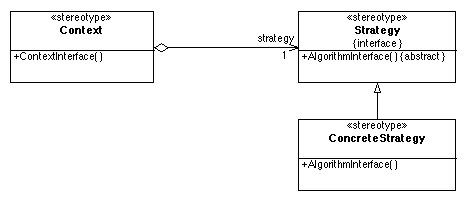
\includegraphics[width=\textwidth]{../diagrams/uml/StrategyPattern.png}
	\caption{Strategie UML}
	\floatfoot{Source: (../diagrams/uml~commonswiki, Commons-Wiki, 11 Jul 2017)}
\end{figure}

\newpage
\subsection{Dekorierer}

\textit{engl. Decorator pattern}

\begin{defi}
	Der \textbf{Dekorierer} fügt Objekten dynamisch Funktionalität hinzu.
\end{defi}

\begin{ex}[Java]
	Im folgenden Beispiel werden wir Eis mit Extras "dekorieren".
	
	
	\lstinputlisting[language=Java, caption=Erstellen userer zu dekorierenden Schnittstelle Schnittstelle]{../java/examples/decorator/IceCream.java}
	\lstinputlisting[language=Java, caption=Schnittstellen Implementierung]{../java/examples/decorator/GenericIceCream.java}
	\lstinputlisting[language=Java,caption=Dekorierer]{../java/examples/decorator/IceCreamDecorator.java}
	\lstinputlisting[language=Java,caption=Konkrete Implementierung des Dekorierers]{../java/examples/decorator/WithChocolateChips.java}
	\lstinputlisting[language=Java,caption=Weitere konkrete Implementierung des Dekorierers]{../java/examples/decorator/WithCaramel.java}
	\lstinputlisting[language=Java, caption=Verwendung]{../java/examples/decorator/Main.java}
	
\end{ex}

\begin{why}
	Wenn Zusatzoperationen welche nur teilweise auftreten auf weitere Objekte delegiert werden sollen, während alte Objekte Fortbestand haben sollen.
\end{why}
\begin{figure}[H]
	\centering
	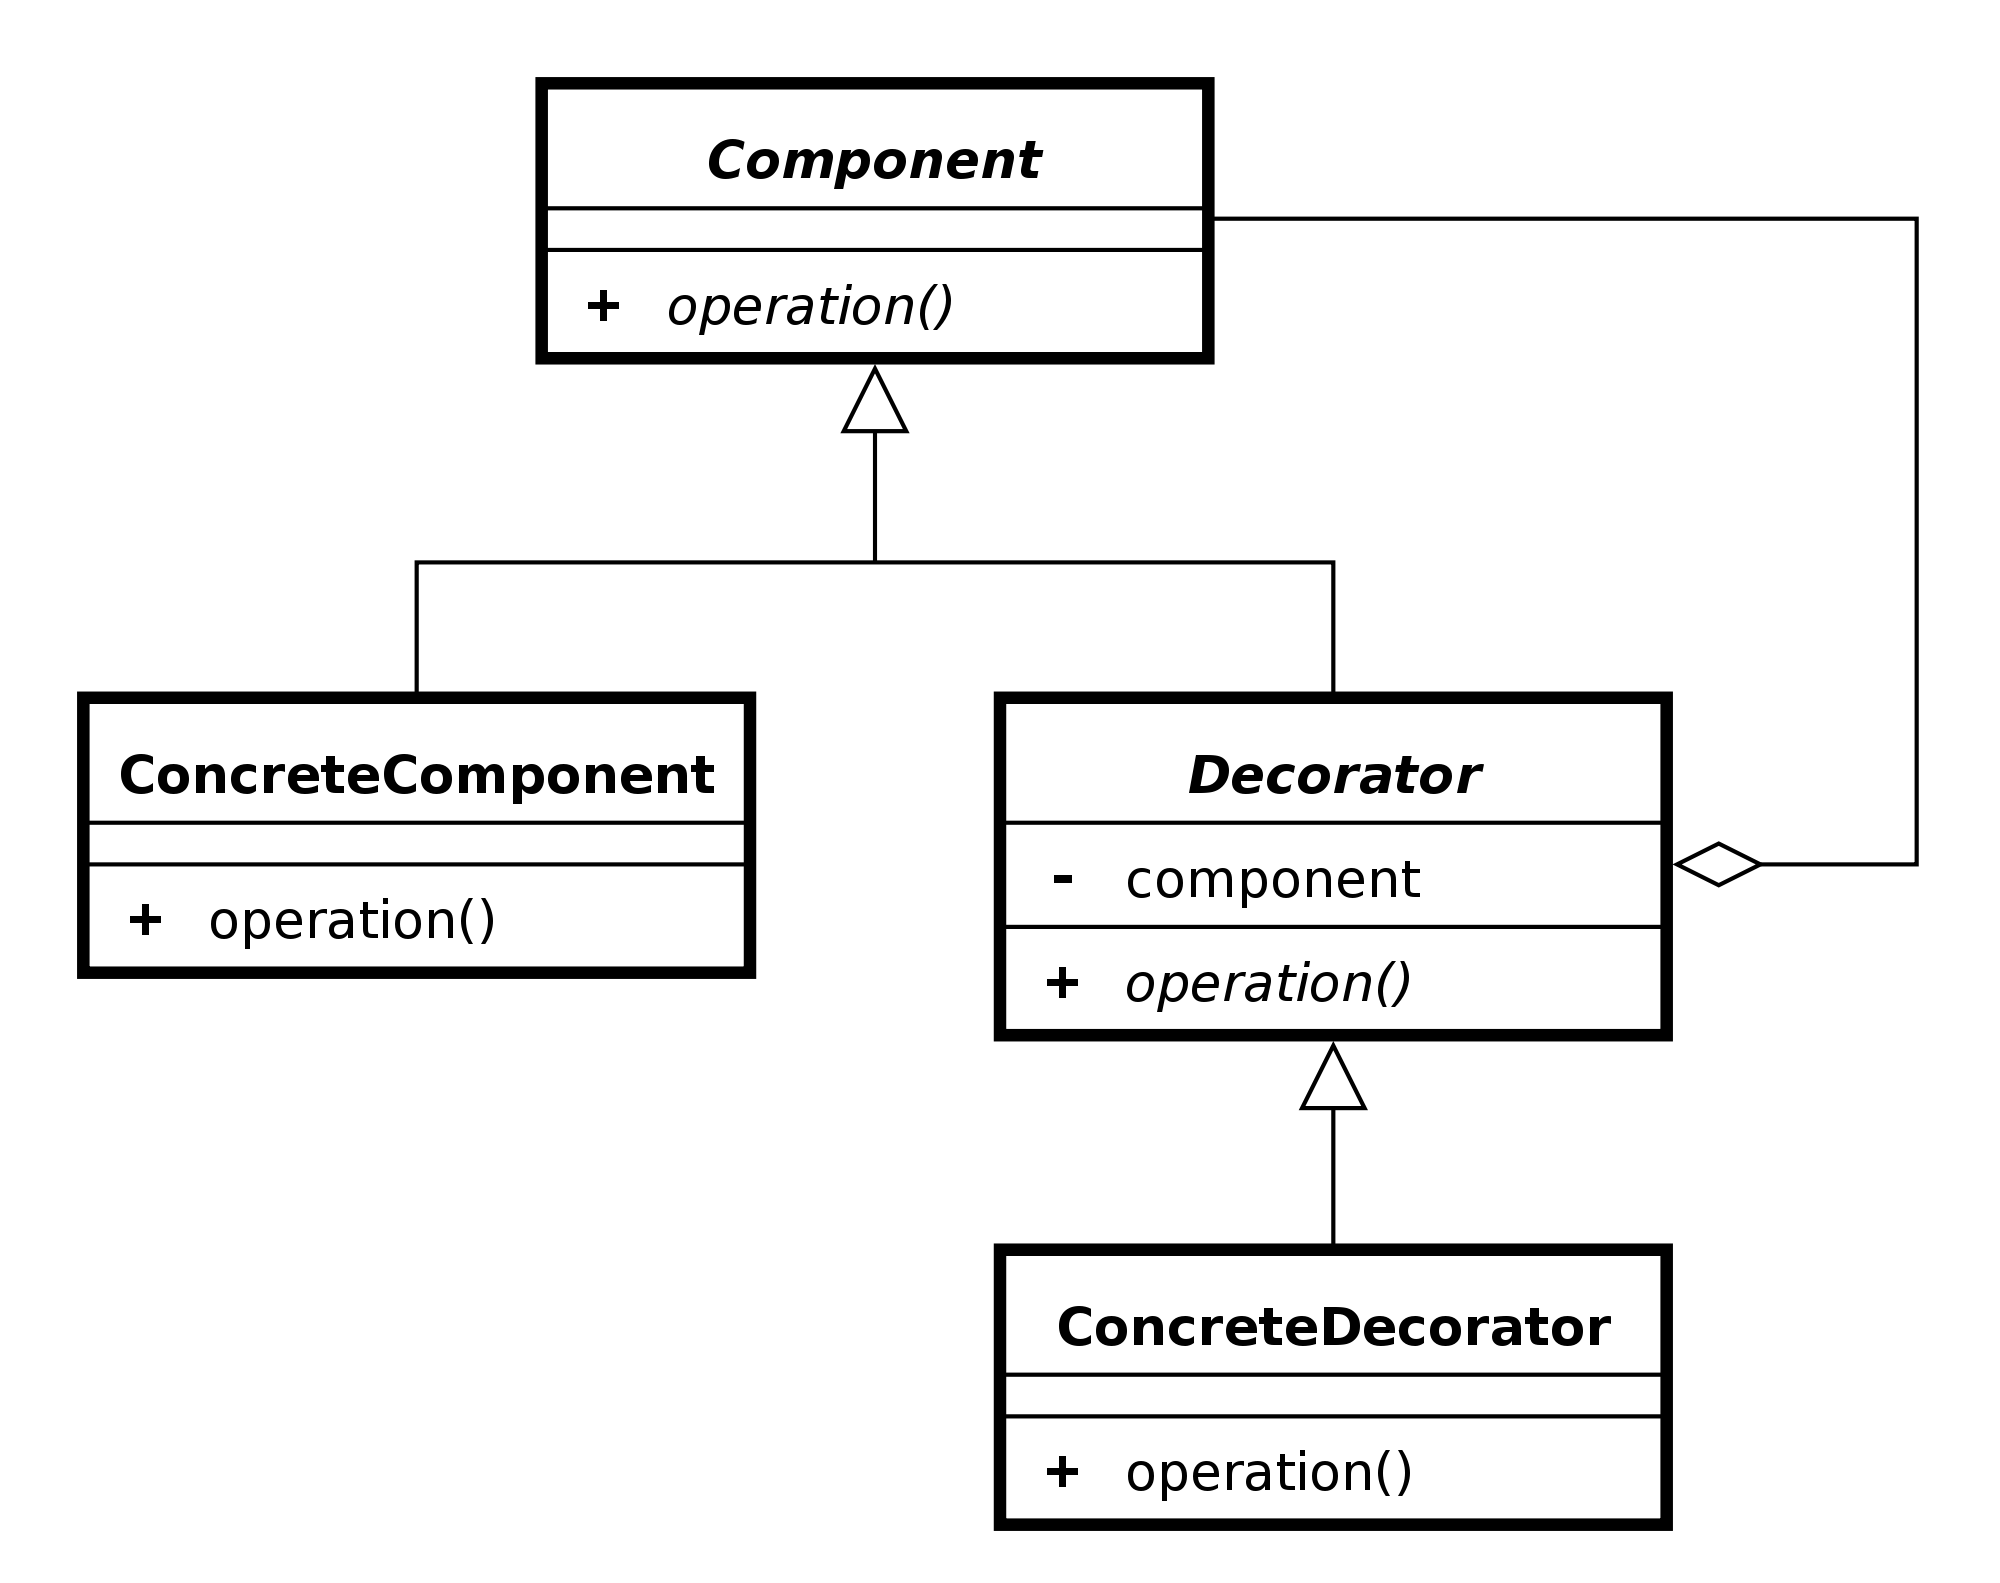
\includegraphics[width=\textwidth]{../diagrams/uml/DecoratorPattern.png}
	\caption{Dekorierer UML}
\end{figure}

\newpage
\subsection{Kompositum}

\textit{engl. Composite pattern}

\begin{defi}
	Ein \textbf{Kompositum} ist eine Gruppe von Objekten, welche genauso behandelt wird wie eine einzelne Instanz des selben Objekttypen
\end{defi}

\begin{ex}[Java API: JComponent]
	In der Java API enthalten ist der JComponent, welcher wiederum weitere Components enthalten kann.
	Zum Beispiel kann ein JPanel ein Label und ein weiteres Panel mit einem Button und einem Bild enthalten und trotzdem wird das obere JPanel genauso als JComponent behandelt wie die einzelnen enthaltenen JComponents behandelt werden (würden).
\end{ex}

\begin{why}
	Wenn Unterscheide zwischen einer einzelnen Ausführung einer Klasse und einer Zusammensetzung dieser für die Verwendung nicht von Relevanz sind.
\end{why}
\begin{figure}[H]
	\centering
	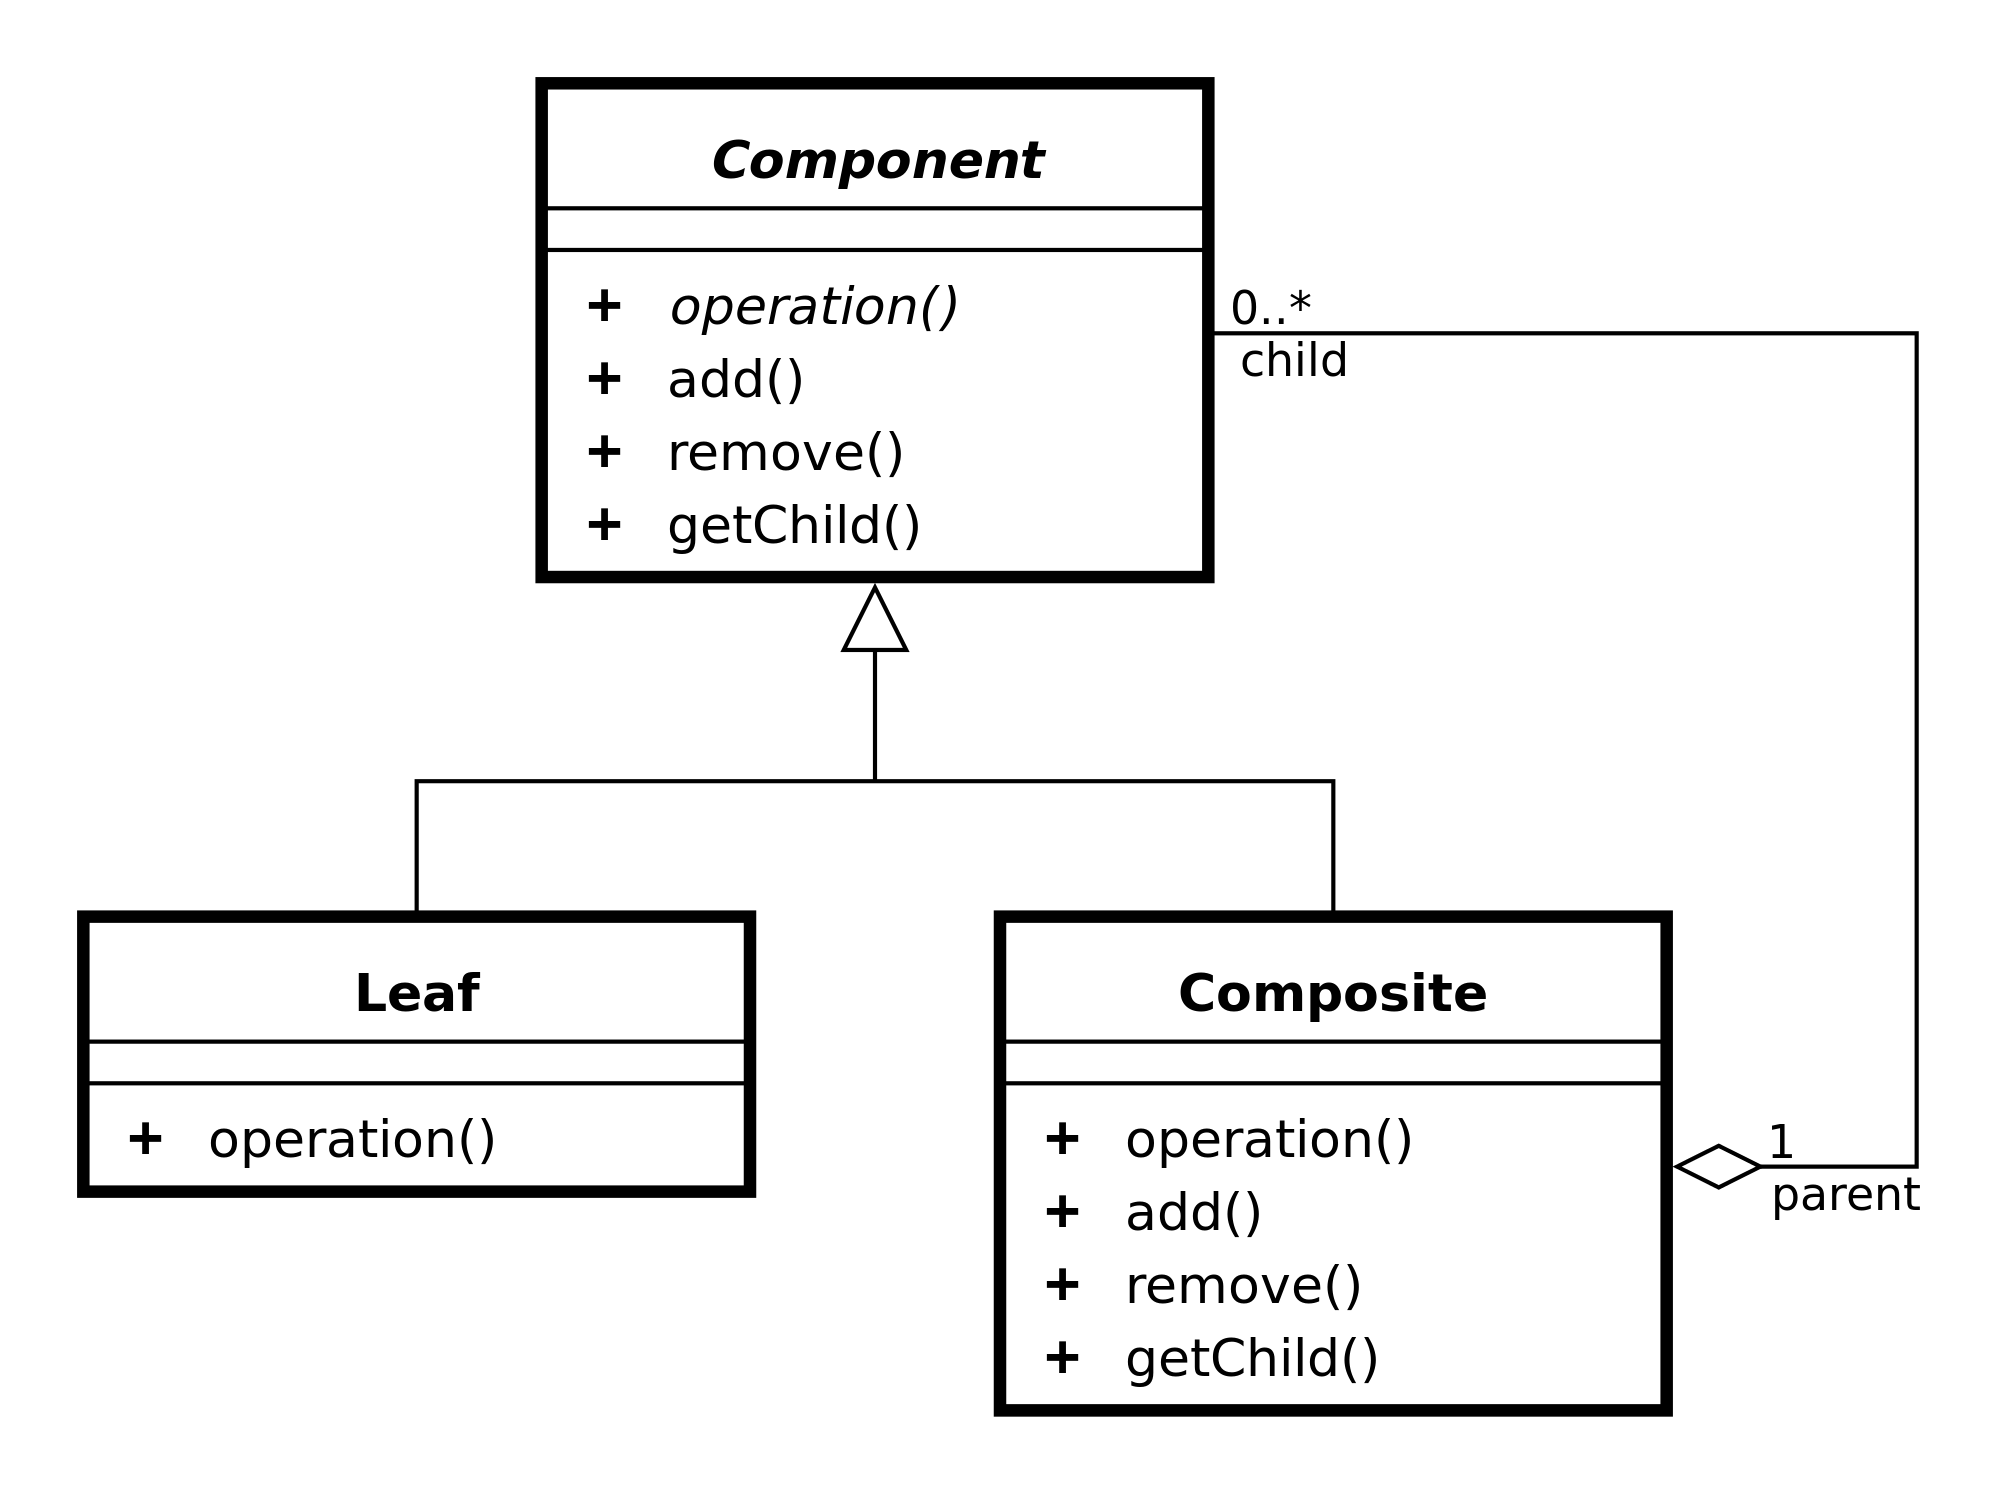
\includegraphics[width=\textwidth]{../diagrams/uml/CompositePattern.png}
	\caption{Kompositum UML}
\end{figure}

\newpage
\subsection{Fabrikmethode}

\textit{engl. Factory Method}

\begin{defi}
	Eine \textbf{Fabrikmethode} ist in einer abstrakte Klasse zur Instanziierung neuer Objekte, welche die konkrete Auswahl der konkreten zu instanziierenden Klasse seinen Unterklassen überlässt.
\end{defi}

\begin{ex}[Java]
	Im folgenden Beispiel werden wir Typen von Studenten ihre Smartphones "bauen" lassen. (Studenten bauen i.A. keine Smartphones, aber es musste ja Beispiel her)

	\lstinputlisting[language=Java, caption=Erstellen unserer Schnittestelle\, von welcher die Subklassen durch die Frabrikmethode gebaut werden sollen Schnittstelle]{../java/examples/factorymethod/Smartphone.java}
	\lstinputlisting[language=Java, caption=1. Schnittstellen Implementierung]{../java/examples/factorymethod/GenericSmartphone.java}
	\lstinputlisting[language=Java, caption=2. Schnittstellen Implementierung]{../java/examples/factorymethod/uPhone.java}
	\lstinputlisting[language=Java,caption=Abstrakte Klasse\, welche durch Fabrikmethode Objekte bauen soll]{../java/examples/factorymethod/Student.java}
	\lstinputlisting[language=Java,caption=Konkrete Implementierung der Klasse mit Fabrikmethode]{../java/examples/factorymethod/NormalStudent.java}
	\lstinputlisting[language=Java,caption=Weitere Implementierung der Klasse mit Fabrikmethode]{../java/examples/factorymethod/BusinessStudent.java}
	\lstinputlisting[language=Java, caption=Verwendung]{../java/examples/factorymethod/Main.java}
\end{ex}

\begin{why}
	\begin{enumerate}
		\item 	Wenn eine Klasse die ihre benötigten zu instanziierenden Objekte nicht kennen kann.
		\item Wenn eine Klasse benötigt, dass ihre Unterklassen Kontrolle über die konkrete Auswahl eines Objekttyps haben müssen.
		\item Zur Insanziierung eines konkreten Objektes welche das Schablonenmethoden Muster verwendet
	\end{enumerate}
\end{why}
\begin{figure}[H]
	\centering
	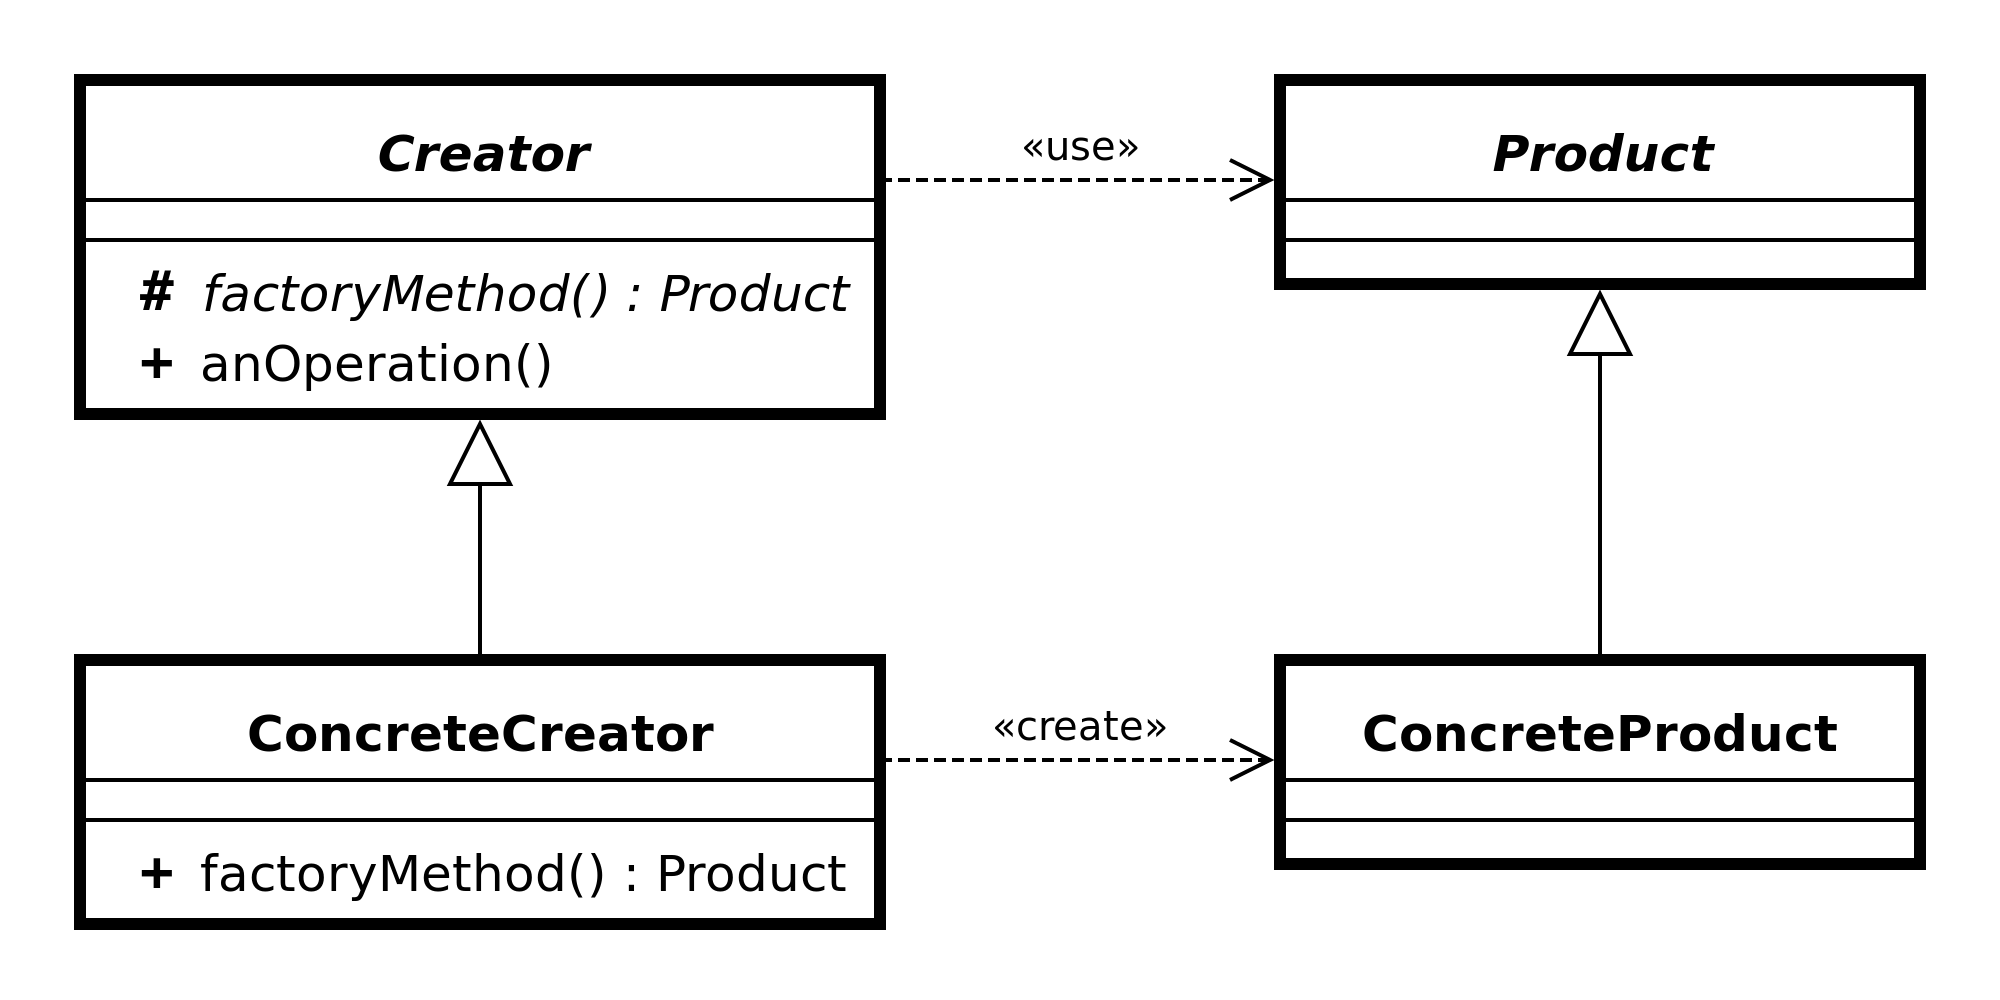
\includegraphics[width=\textwidth]{../diagrams/uml/FactoryMethodPattern.png}
	\caption{Fabrikmethode UML}
\end{figure}


\newpage
\subsection{Schablonen Methode}

\textit{engl. Template Method}

\begin{defi}
	Ein Algorithmen Skelett in einer Operation, welches manche Schritte seien Unterklassen überlässt. (Zu deutsch: Eine Schablonenmethode definiert die Schritte eines Algorithmus, aber überlässt (Teil-)Implementierungen den Unterklassen)
\end{defi}

\begin{ex}[Java]
	Im folgenden Beispiel wollen wir Mate Tee und Kaffee kochen. Folgendes Beispiel wurde adaptiert von E. Freeman, et. al; Head First Design Patterns.
	
	\lstinputlisting[language=Java, caption=Abstrakte Klasse mit Algorithmus\, welcher nicht alle Schritte implementiert]{../java/examples/templatemethod/CaffeineBeverage.java}
	\lstinputlisting[language=Java, caption=1. Konkrete Umsetzung der Klasse mit Schablonenmethode]{../java/examples/templatemethod/MateTea.java}
	\lstinputlisting[language=Java, caption=2. Konkrete Umsetzung der Klasse mit Schablonenmethode]{../java/examples/templatemethod/Coffee.java}
	\lstinputlisting[language=Java, caption=Verwendung]{../java/examples/templatemethod/Main.java}
	
\end{ex}

\begin{why}
		Um einen Algorithmus zu kapseln, für welchen manche Schritte allerdings nicht allgemein implementiert werden sollen/können.	
\end{why}
\begin{figure}[H]
	\centering
	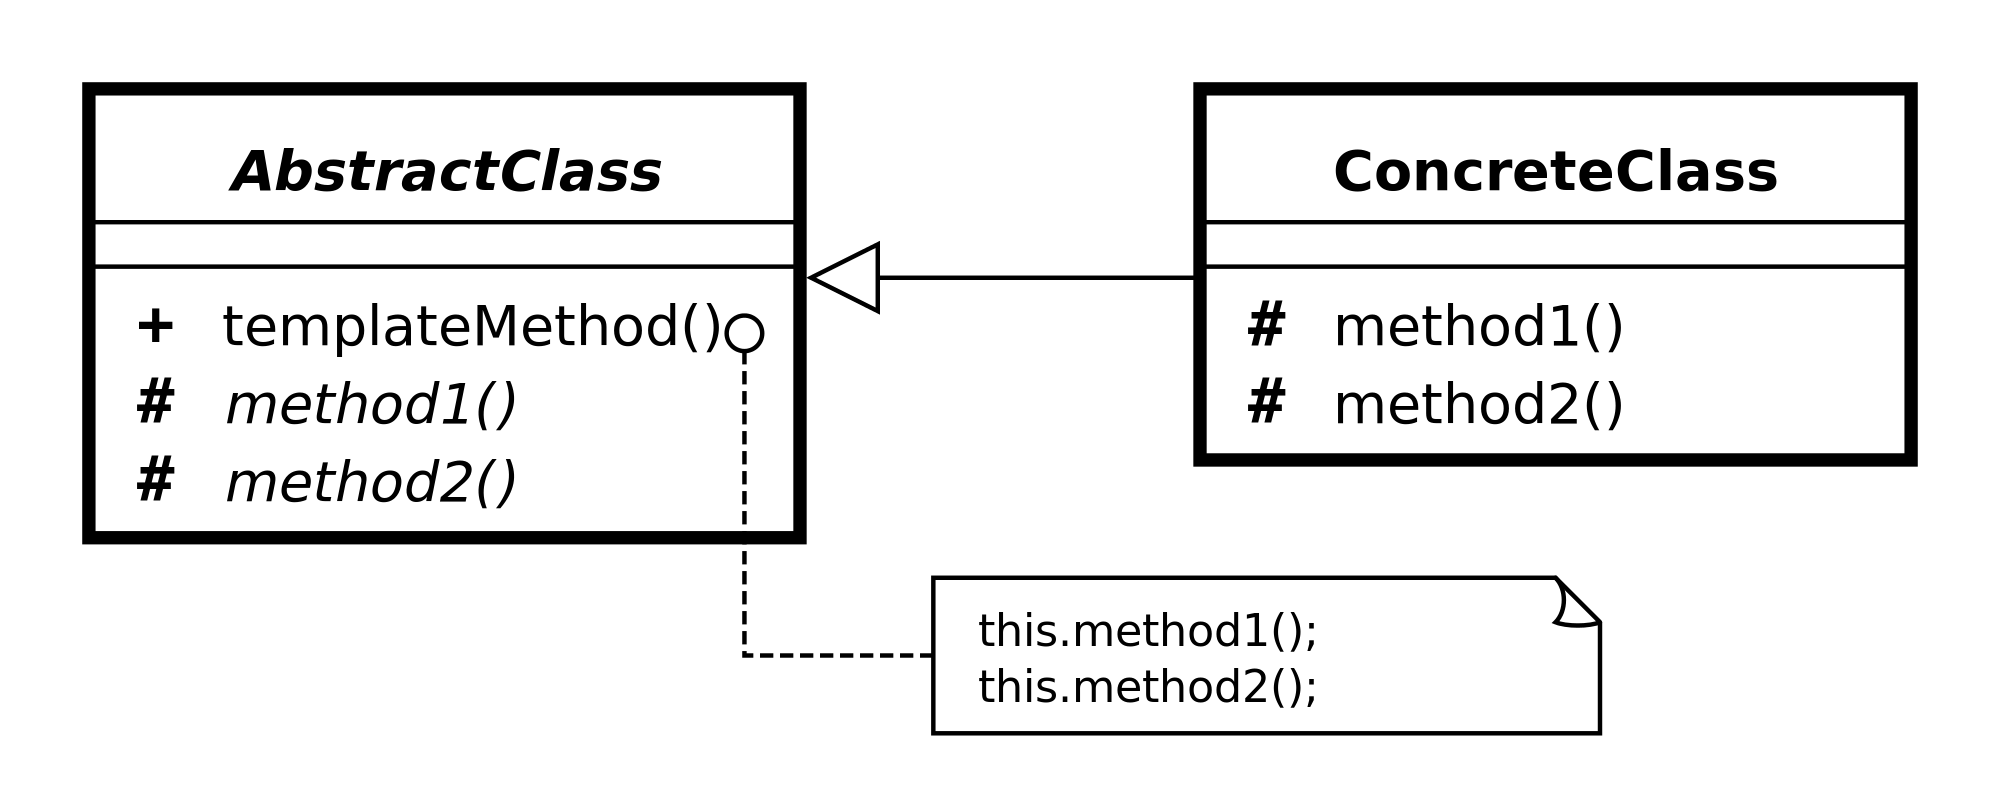
\includegraphics[width=\textwidth]{../diagrams/uml/TemplateMethodPattern.png}
	\caption{Schablonenmethode UML}
\end{figure}


\newpage
\subsection{Besucher}

\textit{engl. Visitor}

\begin{defi}
	Die Kapselung eines auf einer Objektstruktur ausführenden Algorithmus von dieser.
\end{defi}

\begin{ex}[Java]
	Im folgenden Beispiel besuchen wir einen Computer auf verschiedene Arten
	
	\lstinputlisting[language=Java, caption=Zu besuchendes Interface]{../java/examples/visitor/ComputerComponent.java}
	\lstinputlisting[language=Java, caption=Konkrete Umsetzung der zu besuchenden Schnittstelle]{../java/examples/visitor/Computer.java}
	\lstinputlisting[language=Java, caption=Konkrete Umsetzung der zu besuchenden Schnittstelle]{../java/examples/visitor/CPU.java}
	\lstinputlisting[language=Java, caption=Konkrete Umsetzung der zu besuchenden Schnittstelle]{../java/examples/visitor/RAM.java}
	\lstinputlisting[language=Java, caption=Konkrete Umsetzung der zu besuchenden Schnittstelle]{../java/examples/visitor/GraphicsCard.java}
	
	\lstinputlisting[language=Java, caption=Visitorinterface]{../java/examples/visitor/ComputerComponentVisitor.java}
	\lstinputlisting[language=Java, caption=Konkrete Umsetzung der besuchenden Schnittstelle]{../java/examples/visitor/FixVisitor.java}
	\lstinputlisting[language=Java, caption=Konkrete Umsetzung der besuchenden Schnittstelle]{../java/examples/visitor/SpillVisitor.java}
	
	\lstinputlisting[language=Java, caption=Verwendung]{../java/examples/visitor/Main.java}
	
\end{ex}

\begin{why}
	Um das Open-Closed Principle einzuhalten.
\end{why}
\begin{figure}[H]
	\centering
	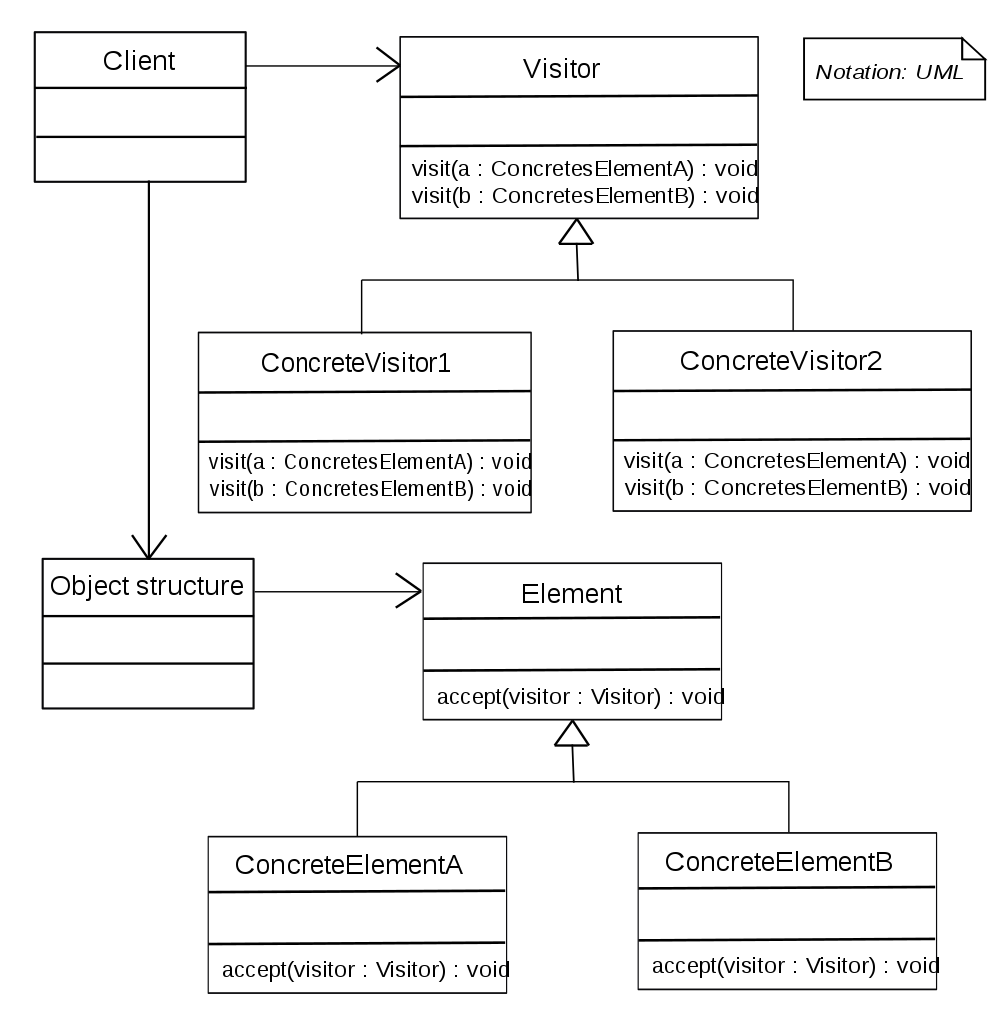
\includegraphics[width=\textwidth]{../diagrams/uml/VisitorPattern.png}
	\caption{Besucher UML}
	\floatfoot{Source: (Sae1962, Commons-Wiki, 11 Jul 2017)}
\end{figure}




\newpage
\subsection{Abstrakte Fabrik}

\textit{engl. Abstract Factory}

\begin{defi}
	Eine \textbf{Abstrakte Fabrik} bietet eine Schnittstelle zur Instanziierung von Familien bestehend aus voneinander abhängigen Objekten
\end{defi}

\begin{ex}[Java]
	Im folgenden Beispiel besuchen wir einen Computer auf verschiedene Arten
	
	\lstinputlisting[language=Java, caption=Die abstrakte Fabirk]{../java/examples/abstractfactory/GUIFactory.java}
	\lstinputlisting[language=Java, caption=Konkrete Umsetzung der Fabrik]{../java/examples/abstractfactory/OSXGUIFactory.java}
	\lstinputlisting[language=Java, caption=Konkrete Umsetzung der Fabrik]{../java/examples/abstractfactory/LinuxGUIFactory.java}
	\lstinputlisting[language=Java, caption=Konkrete Umsetzung der Fabrik]{../java/examples/abstractfactory/WindowsGUIFactory.java}
	
	
	\lstinputlisting[language=Java, caption=Das zu erstellende Interface]{../java/examples/abstractfactory/NavBar.java}
	
	
	\lstinputlisting[language=Java, caption=Verwendung]{../java/examples/abstractfactory/Main.java}
	
\end{ex}

\begin{why}
	\begin{enumerate}
		\item Um eine System unabhängig von seiner Produkterzeugung sein soll
		\item Wenn eine Familie von aufeinander abgestimmten Produkten benötigt wird
		\item Bei einer Bibliothek welche keine Implementierungen, sondern nur Schnittstellen offen legen soll
	\end{enumerate}
	
	
\end{why}
\begin{figure}[H]
	\centering
	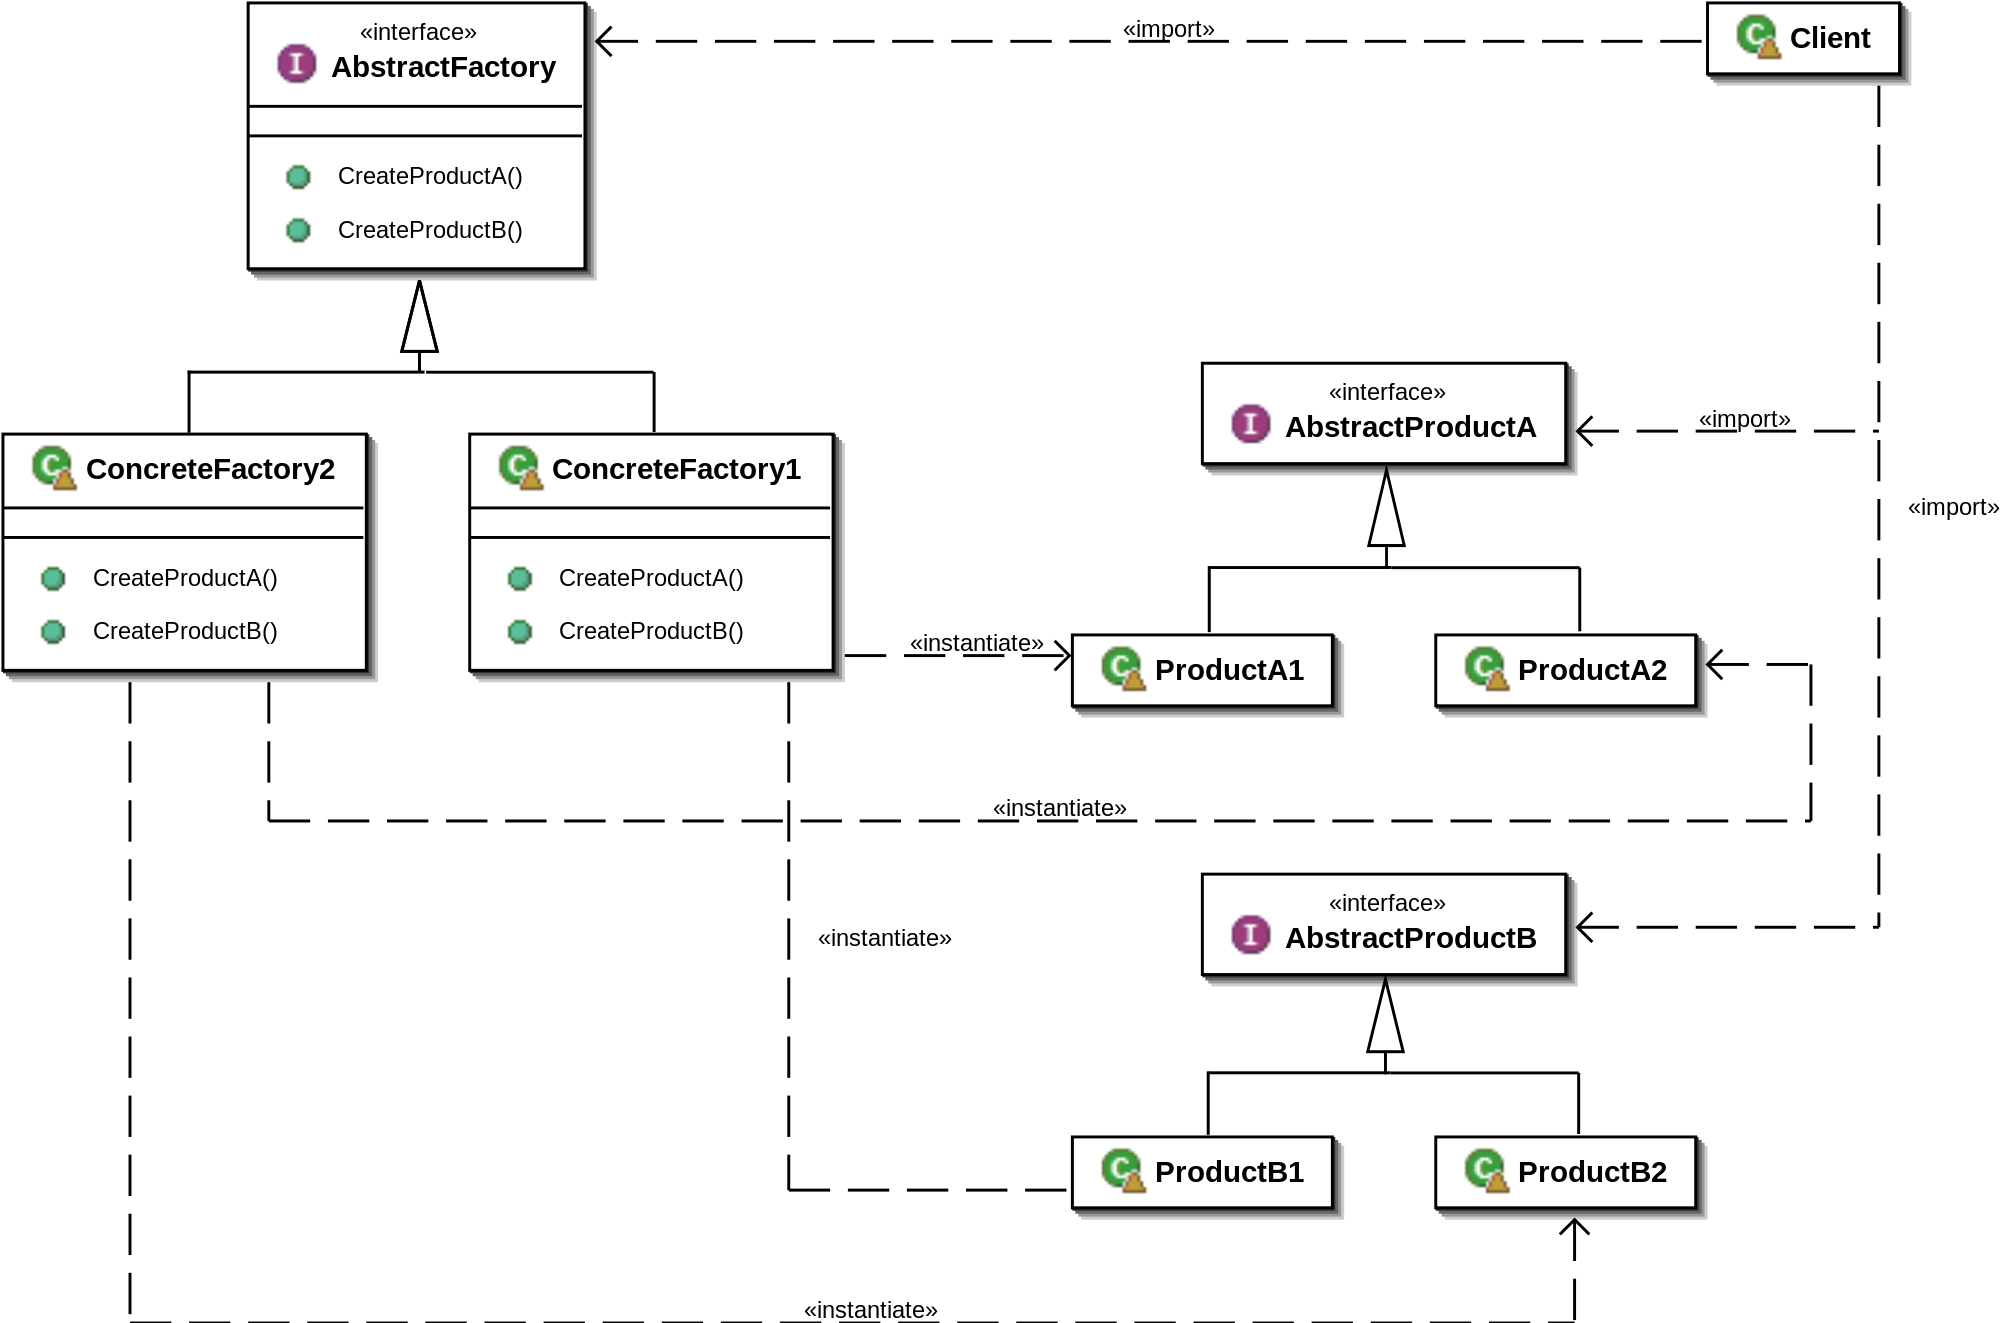
\includegraphics[width=\textwidth]{../diagrams/uml/AbstractFactoryPattern.png}
	\caption{Abstrakte Fabrik UML}
	\floatfoot{Source: (Giacomo Ritucci, Commons-Wiki, 11 Jul 2017)}
\end{figure}


\newpage


\section{Entkopplungsmuster}
\subsection{Adapter}
\textit{engl. bzw. allgemein verständlich: Wrapper}
\begin{defi}
	Ein \textbf{Adapter} passt eine vorh. Schnittstelle an eine benötigte Schnittstelle an
\end{defi}
\begin{ex}[Java]
	Java Integer, Double, etc. (Notice captials)
\end{ex}
\begin{why}
	\begin{enumerate}
		\item Wenn eine Klasse welche benötigt ist nicht der benötigten Schnittstelle entspricht
		\item Wenn eine Klasse mit unbekannten Klassen zsm arbeiten soll, von welchen man allerdings noch nicht die benötigten Schnittstellen kennt
		\item Wenn es unpraktisch ist Schnittstellen für Unterklassen anzupassen
	\end{enumerate}
\end{why}
\begin{figure}[H]
	\centering
	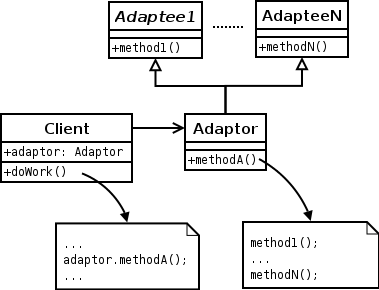
\includegraphics[width=\textwidth]{../diagrams/uml/AdapterPattern.png}
	\caption{Adapter UML}
\end{figure}

\newpage
\subsection{Beobachter}
\textit{engl. bzw. allgemein verständlich: Observer}
\begin{defi}
	Ein \textbf{Beobachter} definiert eine 1-zu-n Abhängigkeit zw. Objekten, so dass Änderung des einen Objektes zu einer Benachrichtigung und ggf. einer Aktualisierung der n Objekte führt.
\end{defi}
\begin{ex}[Java]
	In diesem Beispiel fragen wir den Nutzer wie es ihm geht und geben jeweils seine Antwort aus. Bitte beachte: Die abstrakten Klassen (siehe UML) stammen hier aus der Java-API
	
	\lstinputlisting[language=Java, caption=Das konkrete Subjekt]{../java/examples/observer/InputSubject.java}
	\lstinputlisting[language=Java, caption=Verwendung des Beochbachters auf das Subjekt]{../java/examples/observer/QuestionAsker.java}
\end{ex}
Bitte beachten: Im obrigen Beispiel wurden Daten an den Beobachter geliefert, dies ist i.A. nicht der Fall (siehe UML).
\begin{why}
	\begin{enumerate}
		\item Subjekt \& Beobachter könnten unabh. voneinander wiederverwendet werden
		\item Beobachter können im "Plug n Play"-Stil hinzugefügt und entfernt werden
		\item Verhindert Zyklen in der Benutzthierarchie: Der Beobachter beobachtet ein unbekanntes Subjekt und das Subjekt hat n Beobachter
		\item Änderungen können schnell anderen Teilen der Software bekannt gemacht werden
		\item u. U. können auch Daten an den Beobachter geliefert werden um so auf bestimmte Aktionen reagieren zu können (häufig der Fall)
		\item Nützlich in asynchronen Anwendungen (z.B. RSS)
	\end{enumerate}
\end{why}
\begin{figure}[H]
	\centering
	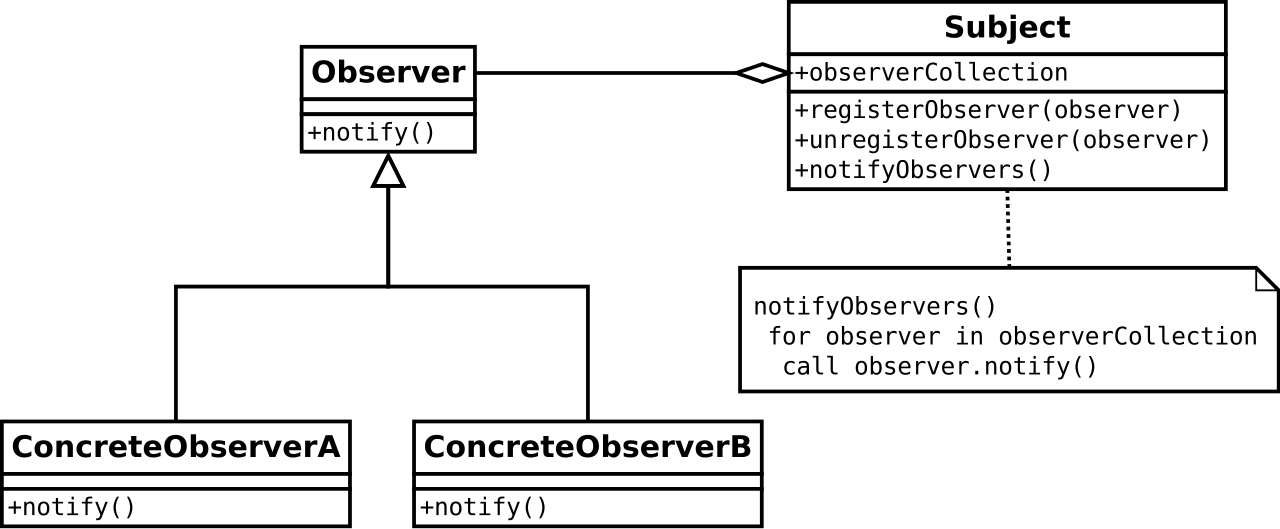
\includegraphics[width=\textwidth]{../diagrams/uml/ObserverPattern.png}
	\caption{Beobachter UML}
\end{figure}

\newpage
\subsection{Brücke}
\textit{engl. Bridge o. Handle}
\begin{defi}
	Eine \textbf{Brücke} entkoppelt die Abstraktion von ihrer Implementierung
\end{defi}
\begin{ex}[Nicht vorh.]
\end{ex}
\begin{why}
	\begin{enumerate}
		\item Unterklassenbildung auf sowohl Abstraktion und Implementierung möglich
		\item Änderung einer Implementierung hat nicht unbedingt Einfluss auf Klienten
		\item Verdeckt Implementierung vollst. vom Klienten
		\item Spart u. U. bei Anzahl der Klassen
	\end{enumerate}
\end{why}
\begin{figure}[H]
	\centering
	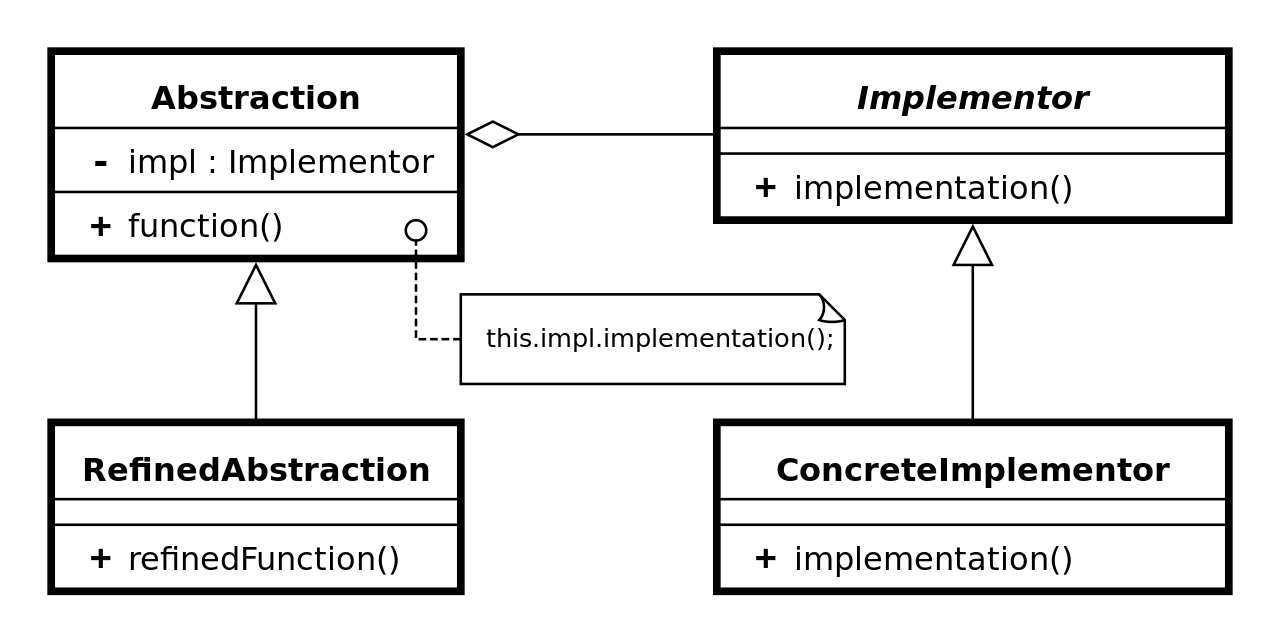
\includegraphics[width=\textwidth]{../diagrams/uml/BridgePattern.png}
	\caption{Brücke UML}
\end{figure}

\newpage
\subsection{Iterator}

\begin{defi}
	Ein \textbf{Iterator} ermöglicht sequenziellen Zugriff auf Objekte, ohne ihre zugrundeliegende Repräsentation offen zu legen.
\end{defi}
\begin{ex}[Java]
	Siehe java.util.Iterator \& java.util.Collection
\end{ex}
\begin{why}
	\begin{enumerate}
		\item Bietet eine einheitliche Schnittstelle zur sequenziellen Traversierung verschiedener Datenstrukturen
		\item Mit mehreren Iteratoren kann man gleichzeitig auf verschiedene Objekte zugreifen (Robustheit)
	\end{enumerate}
\end{why}
\begin{figure}[H]
	\centering
	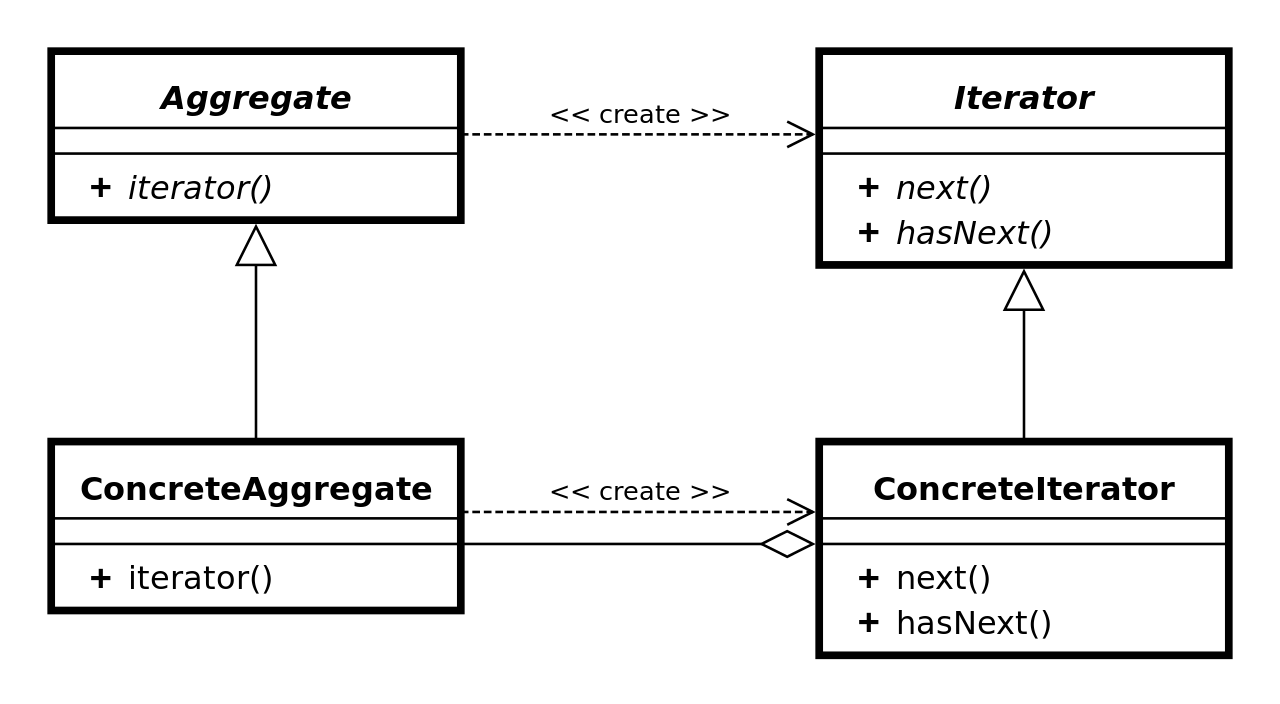
\includegraphics[width=\textwidth]{../diagrams/uml/IteratorPattern.png}
	\caption{Iterator UML}
\end{figure}

\newpage
\subsection{Stellvertreter}
\textit{engl. Proxy}
\begin{defi}
	Eine \textbf{Stellvertreter} kontrolliert den Zugriff auf ein Objekt
\end{defi}

Es gibt weiterhin spezielle Typen Stellvertreter:
\begin{enumerate}
	\item \textbf{Protokollierender Stellvertreter:}\newline
	 Ein protokollierender Stellvertreter zählt Referenzen auf das	eigentliche Objekt, so dass es automatisch freigegeben werden kann, wenn keine Referenzen mehr auf das Objekt existieren. Er kann auch andere Zugriffsinformationen protokollieren und leitet Zugriffe weiter. 
	\item \textbf{Puffernder Stellvertreter:}\newline
	Ein puffernder Stellvertreter (\textit{engl. caching proxy}) lädt ein persistentes Objekt erst dann in den Speicher, wenn es das erste Mal angesprochen wird. Er kann auch einen Puffer mit mehreren Objekten verwalten, die nach Bedarf zwischen Hintergrund- und Hauptspeicher bewegt werden.
	\item \textbf{Fernzugriffsvertreter:}\newline
	Ein Fernzugriffsvertreter (\textit{engl. remote proxy}) stellt einen lokalen Stellvertreter für ein Objekt in einem anderen Adressraum dar.
\end{enumerate} 
\begin{ex}[Java]
	//TODO
\end{ex}
\begin{why}
	\begin{enumerate}
		\item Falls eine funktionsreichere Referenz auf ein Objekt als ein Zeiger benötigt wird
	\end{enumerate}
\end{why}
\begin{figure}[H]
	\centering
	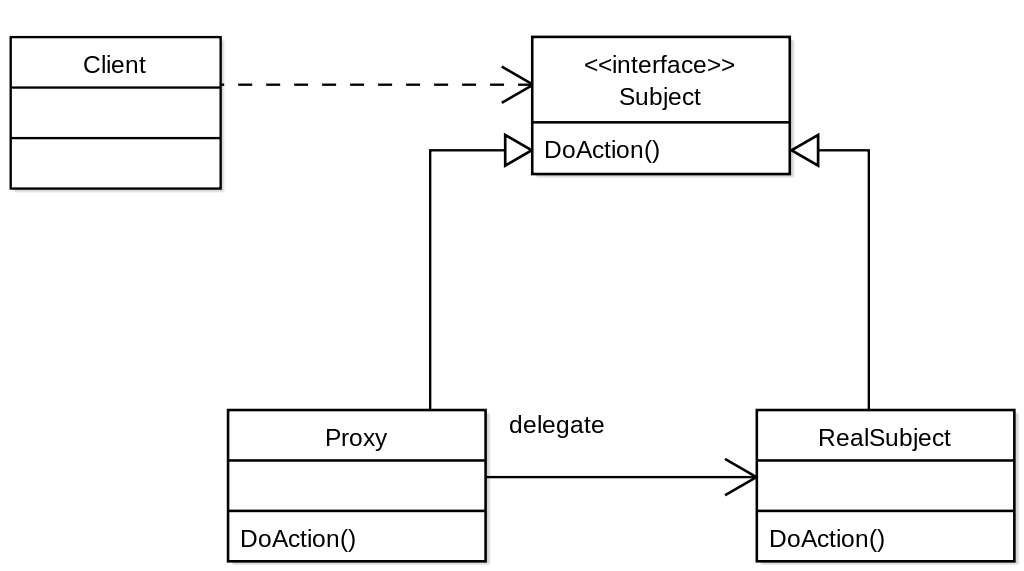
\includegraphics[width=\textwidth]{../diagrams/uml/ProxyPattern.png}
	\caption{Proxy UML}
\end{figure}

\newpage
\subsection{Vermittler}
\textit{engl. Mediator}
\begin{defi}
	Ein \textbf{Vermittler} kapselt das Zusammenspiel einer Menge von Objekten in sich.
\end{defi}
\begin{ex}[Java]
	//TODO
\end{ex}
\begin{why}
	\begin{enumerate}
		\item Vermittler fördern lose Kopplung, indem sie Objekte davon	abhalten, aufeinander explizit Bezug zu nehmen
		\item Wenn ein Objekt sich auf zu viele Objekte bezieht, kann dieses Muster als Gegenmaßnahme verwendet werden und somit Wiederverwendbarkeit erhöhen
		\item Wenn eine Menge von Objekten vorliegt, die in wohldefinierter, aber komplexer Weise zusammen arbeiten.
		\item Wenn ein auf mehrere Klassen verteiltes Verhalten maßgeschneidert werden soll, ohne viele Unterklassen bilden zu müssen.
	\end{enumerate}
\end{why}
\begin{figure}[H]
	\centering
	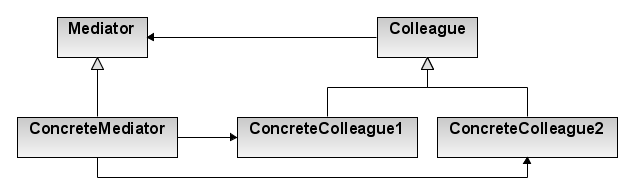
\includegraphics[width=\textwidth]{../diagrams/uml/MediatorPattern.png}
	\caption{Vermittler UML}
\end{figure}

\newpage
\section{Zustandshandhabungsmuster}
\subsection{Einzelstück}
\textit{engl. singleton}
\begin{defi}
	Ein \textbf{Einzelstück} sichert die Alleinexistenz eines gegebenen Objektes zu
\end{defi}
\begin{ex}[Java]
		\lstinputlisting[language=Java, caption=Einzelstück]{../java/examples/singleton/UniqueItem.java}
\end{ex}
\begin{why}
	\begin{enumerate}
		\item Ein Einzelstück stellt sicher, dass wenn es nicht klar ist in welchem Teil der Software ein Objekt zuerst erstellt wird, dass es weiterhin nur eines gibt
		\item Um eine Klasse um eine einzige Instanz zu limitieren und einen zentralen Abrufpunkt zu bieten
		\item Es kann die einzige Instanz durch Unterklassenbildung
		erweiterbar sein und die Klienten diese ohne Veränderung
		ihres Quelltextes nutzen
	\end{enumerate}
\end{why}
\begin{figure}[H]
	\centering
	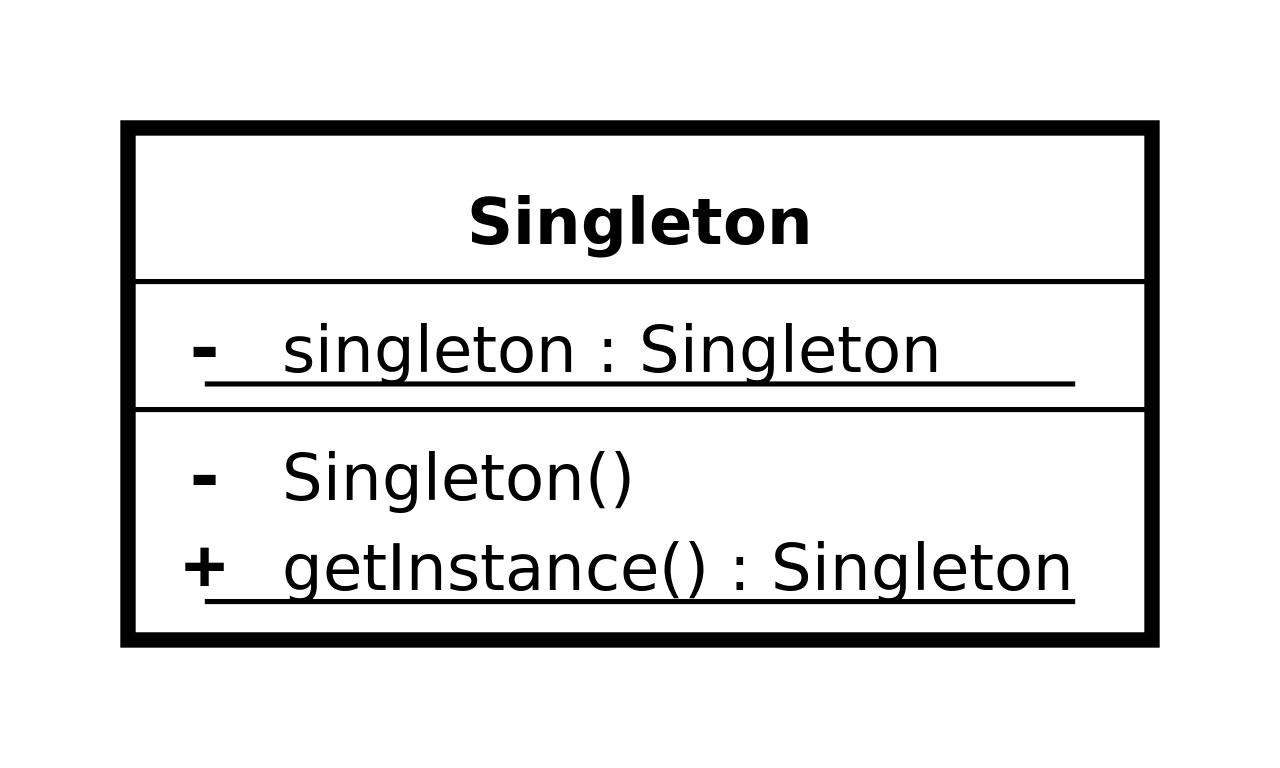
\includegraphics[width=\textwidth]{../diagrams/uml/SingletonPattern.png}
	\caption{Einzelstück UML}
\end{figure}


\newpage
\subsection{Fliegengewicht}
\textit{engl. flyweight}
\begin{defi}
	Ein \textbf{Fliegengewicht} minimiert Datennutzung durch Datenteilung mit anderen Objekten
\end{defi}
\begin{ex}[Java]
	\lstinputlisting[language=Java, caption=Fliegengewicht (Source: \"Fliegengewicht (Entwurfsmuster).\" Wikipedia. Wikimedia Foundation 28 June 2017. Web. 22 July 2017)]{../java/examples/flyweight/Flyweight.java}
	
\end{ex}
\begin{why}
	\begin{enumerate}
		\item Löst das Problem, dass Objekte auf Grund ihrer Anzahl bereits viel Speicher verbrauchen
		\item Um den Objektzustand aus dem Objekt zu ziehen
		\item Ersetzt viele Gruppen von Objekten durch relativ wenige gemeinsam genutzte Objekte
	\end{enumerate}
	\textbf{N.B.:} Dies geht nur wenn die Anwendung nicht von der Identität der Objekte abhängt
\end{why}
\begin{figure}[H]
	\centering
	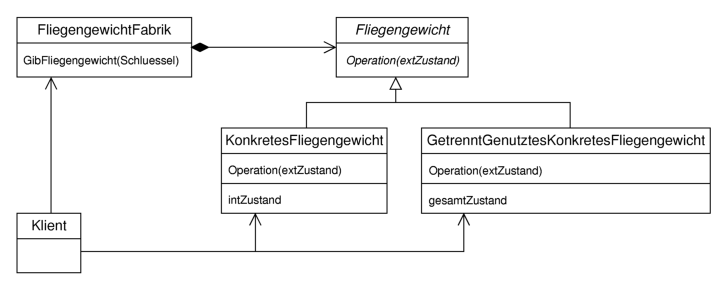
\includegraphics[width=\textwidth]{../diagrams/uml/FlyweightPattern.png}
	\caption{Flyweight UML}
	\floatfoot{Source: (Thomasv, Wikimedia, 22 Jul 2017)}
\end{figure}


\newpage
\subsection{Memento}
\textit{engl. Memento or Token}
\begin{defi}
	Das Muster \textbf{Memento} dient der Erfassung und Externalisierung des internen Zustands eines Objektes, wobei sichergestellt wird, dass dadurch seine Kapselung nicht verletzt wird. So kann das Objekt zu einem späteren Zeitpunkt wieder in diesen Zustand zurückversetzt werden.
\end{defi}
\begin{ex}[Java]
		\lstinputlisting[language=Java, caption=HistoricalText: Eine Klasse mit Mementoverwendung]{../java/examples/memento/HistoricalText.java}
		\bigskip % To prevent 2 lines on prev page
		\lstinputlisting[language=Java, caption=Wrapper von HistoricalText\, welcher zusätzlich die Mementos speichert]{../java/examples/memento/TextStorer.java}
		\lstinputlisting[language=Java, caption=Verwendung mit Nutzerschnittstelle]{../java/examples/memento/Main.java}
\end{ex}
\begin{why}
	\begin{enumerate}
		\item Erlaubt das Zwischenspeichern einer Momentaufnahme und das spätere Zurücksetzen auf diese (z.B. (CMD/Ctrl) + Z \& Spielspeicherstände)
		\item Kapselt weiterhin, wenn einer direkte Schnittstelle zum ermitteln des Zustands die nicht tun würde
	\end{enumerate}
\end{why}
\begin{figure}[H]
	\centering
	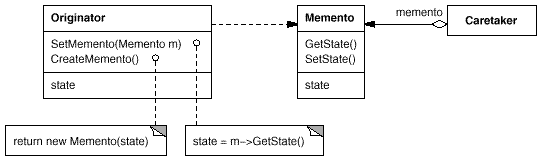
\includegraphics[width=\textwidth]{../diagrams/uml/MementoPattern.png}
	\caption{Memento UML}
	\floatfoot{Source: (Kholodov, Igor. "Design Patterns." CIS-75 Software Specification and Design. Bristol Community College: Computer Information Systems Department, n.d. Web. 23 July 2017.)}
\end{figure}

\newpage
\subsection{Prototyp}
\textit{engl. Prototype}
\begin{defi}
	Das Muster \textbf{Prototyp} lässt neue Instanzen basierend auf einer Vorlage erzeugen
\end{defi}
\begin{ex}[Java]
	java.lang.Object\#clone()
\end{ex}
\begin{why}
	\begin{enumerate}
		\item Falls der Objektbau länger dauert als eine Kopie
		\item Um eine Klassenhierarchie von Fabriken zu vermeiden
		\item Wenn Exemplare einer Klasse nur wenige Zustandskombinationen haben können. i.d.F. Kann man die Prototypen anlegen und kopieren
	\end{enumerate}
\end{why}
\begin{figure}[H]
	\centering
	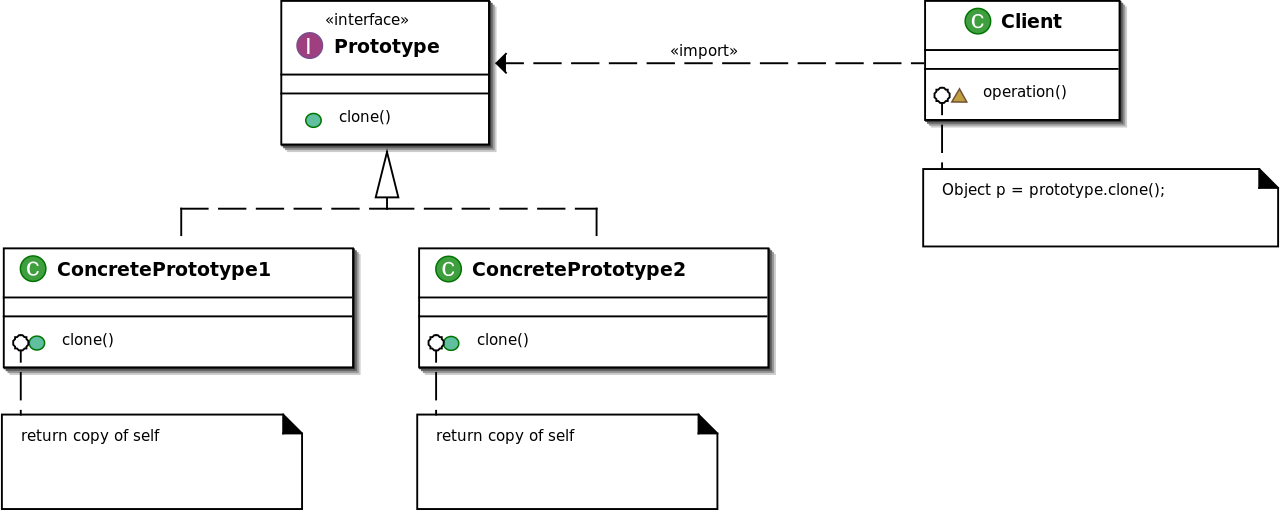
\includegraphics[width=\textwidth]{../diagrams/uml/PrototypePattern.png}
	\caption{Prototyp UML}
	\floatfoot{Source: (Wikimedia commons - Giacomo Ritucci. 23.07.2017)}
\end{figure}

\newpage
\subsection{Zustand}
\textit{engl. State}
\begin{defi}
	Das Muster \textbf{Zustand} implementiert einen Zustandsautomaten, welcher die Funktionalität basierend auf des Objekts aktuellen Zustand ändert
\end{defi}
\begin{ex}[N/V]
\end{ex}
\begin{why}
	\begin{enumerate}
		\item Das Zustandsmuster wird verwendet, wenn das Verhalten	des Objektes von dessen Zustand abhängt und das Objekt sein Verhalten während der Laufzeit, abhängig vom aktuellen Zustand, ändern muss.
	\end{enumerate}
\end{why}
\begin{figure}[H]
	\centering
	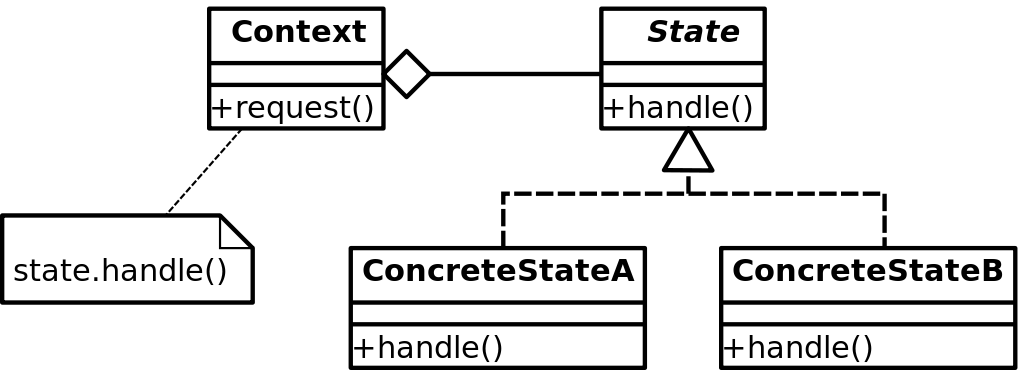
\includegraphics[width=\textwidth]{../diagrams/uml/StatePattern.png}
	\caption{Zustand UML}
	\floatfoot{Source: (Wikimedia commons - JoaoTrindade, apdapted by Ertwroc. 23.07.2017)}
\end{figure}

\newpage
\section{Steuerungsmuster}
\subsection{Befehl}
\textit{engl. Command}
\begin{defi}
	Das Muster \textbf{Befehl} kapselt und parametrisiert alle nötigen Informationen, welche zur Ausführung einer Aktion oder zum auslösen eines Ereignisses benötigt werden.
\end{defi}
\begin{ex}[Java]
	\lstinputlisting[language=Java, caption=Der Befehl]{../java/examples/command/Command.java}

	\lstinputlisting[language=Java, caption=Aufrufer der Kommandos]{../java/examples/command/CommandHandler.java}
	\lstinputlisting[language=Java, caption=Verwendung mit Nutzerschnittstelle]{../java/examples/command/Main.java}
\end{ex}
\begin{why}
	\begin{enumerate}
		\item Möglich Aktionen in eine Warteschlange (\textit{engl. Queue}), in ein Logbuch oder ähnliches zu stellen
		\item Möglichkeit einer Undo-Funktion ohne memento
		\item Wenn ein System mittels komplexer Operationen	strukturiert werden soll, die aus primitiven Operationen aufgebaut werden (Makros)
	\end{enumerate}
\end{why}
\begin{figure}[H]
	\centering
	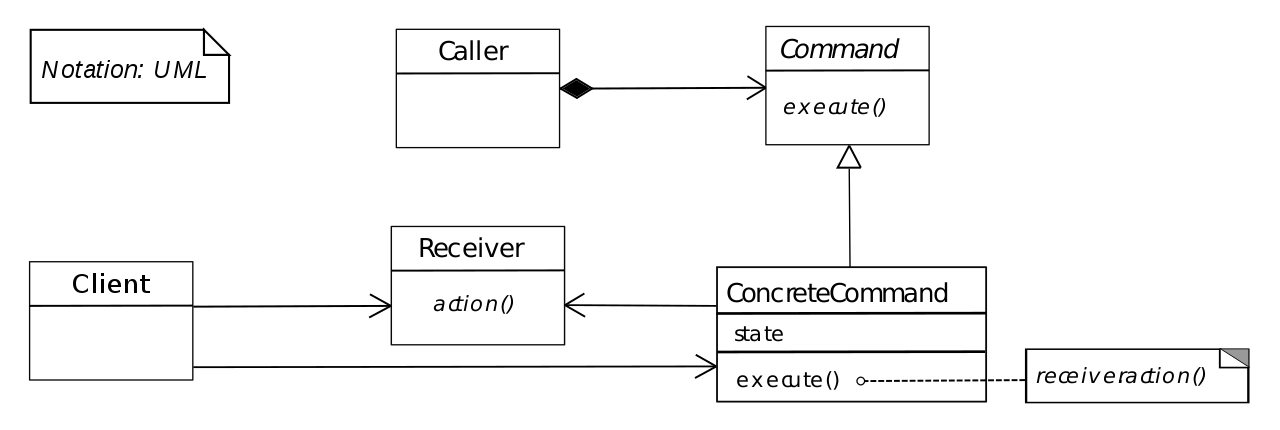
\includegraphics[width=\textwidth]{../diagrams/uml/CommandPattern.png}
	\caption{Befehl UML}
	\floatfoot{Source: (Sae1962, Commons-Wiki, 23 Jul 2017)}
\end{figure}


\newpage
\subsection{Auftraggeber/-nehmer}
\textit{engl. Master/Worker, ehem. Master/Slave}
\begin{defi}
	\textbf{Auftraggeber/-nehmer} bietet fehlertolerante und parallele Berechnung. Ein Auftraggeber verteilt die Arbeit an identische Arbeiter (Auftragnehmer) und berechnet das Endergebnis aus den	Teilergebnissen, welche die Arbeiter zurückliefern.
\end{defi}
\begin{ex}[Allgemein]
	Bildberechnung: Mehrere Fäden (\textit{engl. Threads}) verändern jeweils ein Teil des Bildes mittels des gleichen Algorithmus
\end{ex}
\begin{why}
	\begin{enumerate}
		\item Parallelisierung: Ein Auftraggeber kann Arbeit auf viele Auftragnehmer verteilen, welche auf verschiedenen Fäden (\textit{engl. Threads}) laufen
		\item Lastverteilung (\textit{engl. Load balancing}) möglich
	\end{enumerate}
\end{why}


\newpage
\section{Bequemlichkeitsmuster}
\subsection{Bequemlichkeitsklasse}
\textit{engl. convenience class}
\begin{defi}
	Das Muster \textbf{Bequemlichkeitsklasse} vereinfacht den Methodenaufruf durch Bereithaltung der
	Parameter in einer speziellen Klasse
\end{defi}
\begin{ex}[Java]
	\lstinputlisting[language=Java, caption=Die Bequemlichkeitsklasse]{../java/examples/convclass/Multiply.java}

\end{ex}
\begin{why}
	\begin{enumerate}
		\item Erspart Schreibarbeit und Wiederholungen
	\end{enumerate}
\end{why}
\newpage
\subsection{Bequemlichkeitsmethode}
\textit{engl. convenience method}
\begin{defi}
	Das Muster \textbf{Bequemlichkeitsmethode} vereinfacht den Methodenaufruf durch die Bereitstellung häufig
	genutzter Parameterkombinationen in zusätzlichen Methoden
	(Überladen)
\end{defi}
\begin{ex}[Java]
	\lstinputlisting[language=Java, caption=Die Bequemlichkeitsmethode]{../java/examples/convmethod/Multiply.java}
\end{ex}
\begin{why}
	\begin{enumerate}
		\item Erspart Schreibarbeit und Wiederholungen
	\end{enumerate}
\end{why}
\newpage
\subsection{Fassade}

\begin{defi}
	Das Muster \textbf{Fassade} bietet eine einheitliche Schnittstelle zu einer Menge von Schnittstellen eines Subsystems.\newline
	Die Fassadenklasse definiert eine abstrakte Schnittstelle, welche
	die Benutzung des Subsystems vereinfacht
\end{defi}
\begin{ex}[N/V]
\end{ex}
\begin{why}
	\begin{enumerate}
		\item Bietet einfache Sicht auf das Subsystem
		\item Die
		Einführung einer Fassade entkoppelt die Subsysteme von Klienten und anderen Subsystemen
	\end{enumerate}
\end{why}

\newpage
\subsection{Nullobjekt}

\begin{defi}
	Das Muster \textbf{Nullobjekt} stellt einen Stellvertreter zur Verfügung, der die gleiche
	Schnittstelle bietet, aber nichts tut.
\end{defi}
\begin{ex}[N/V]
\end{ex}
\begin{why}
	\begin{enumerate}
		\item Wenn das Nichtstun von Nöten ist
	\end{enumerate}
\end{why}

\end{document}